\documentclass[12pt,a4paper,twoside,openright]{book}

\usepackage[USenglish,english]{babel}
\usepackage[utf8]{inputenc}

\usepackage{style/isi_style_lt}

\usepackage{amsmath,amsfonts,amssymb,amsthm}
\usepackage{caption}
\usepackage[usenames]{color}
\usepackage{enumerate}
\usepackage{fancyhdr}
\usepackage{fancyvrb}
\usepackage{float}
\usepackage{graphicx}
\usepackage{indentfirst}
\usepackage{listings}
\usepackage{marvosym}
\usepackage{multicol}
\usepackage{sectsty}
\usepackage{subcaption}
\usepackage{tocloft}
\usepackage[table]{xcolor}
\usepackage{url}
\usepackage{longtable}

\AtBeginDocument{%
	\renewcommand{\contentsname}{Table of contents}
	\renewcommand\tablename{Table}
	\renewcommand\figurename{Figure}
	\renewcommand{\lstlistingname}{List}
	\renewcommand{\refname}{Ref.}
}

\definecolor{dkgreen}{rgb}{0,0.6,0}
\definecolor{gray}{rgb}{0.5,0.5,0.5}
\definecolor{mauve}{rgb}{0.58,0,0.82}

\lstset{
  frame=single,
  captionpos=b,
  language=Java,
  aboveskip=3mm,
  belowskip=3mm,
  showstringspaces=false,
  columns=flexible,
  basicstyle={\small\ttfamily},
  numbers=none,
  numberstyle=\tiny\color{gray},
  keywordstyle=\color{blue},
  commentstyle=\color{dkgreen},
  stringstyle=\color{mauve},
  breaklines=true,
  breakatwhitespace=true,
  tabsize=3
}

\makeatletter
\def\cleardoublepage{
	\clearpage\if@twoside \ifodd\c@page\else
	\hbox{}
	\thispagestyle{empty}
	\newpage
	\if@twocolumn\hbox{}\newpage\fi\fi\fi
}

\makeatother

\setlength{\textwidth}{14cm}
\setlength{\textheight}{21cm}
\setlength{\footskip}{3cm}

\setlength{\hoffset}{0pt}
\setlength{\voffset}{0pt}

\setlength{\oddsidemargin}{1cm}
\setlength{\evensidemargin}{1cm}

\universita{Alma Mater Studiorum -- Università di Bologna}

\campus{Campus di Cesena}

\scuola{Scuola di Ingegneria e Architettura}

\corsodilaurea{Laurea Magistrale in Ingegneria e Scienze Informatiche}

\titolo{Scala-omg}

\materia{PPS - Paradigmi di programmazione e sviluppo}

\laureando{Gabriele Guerrini, Riccardo Salvatori, Stefano Salvatori}

\annoaccademico{2019 -- 2020}

\makeindex

\begin{document}

\frontmatter 

\maketitle

\tableofcontents

\mainmatter

\pagestyle{fancy} 
\fancyhead[LE,RO]{\thepage}
\fancyfoot{}

\chapter{Scoping}

\section{Introduction}

The deliverable should consist of a library that simplifies the development of distributed client-server applications based upon a concept of room. Videogames largely use rooms in every feature (match, lobby, trading room etc.) but there are lots of potential different domains where such idea can be applied (chatrooms, for instance).
\\
The main idea of the product is to provide a low level support that handles all aspects of communication, so that developers that use the library can focus on program logic itself, without concerning about issues due to networking, serialization, synchronization between clients, integration of clients and rooms, and so on.
\\
Hence, the library provides three main notions of:
\begin{itemize}
\item \textbf{Room}: place where clients can gather to do something.
\item \textbf{Server}: a game server where rooms can be hosted.
\item \textbf{Client}: entity that might do operation on rooms, such as joining, sending messages etc.
\end{itemize} 

\section{System Requirements Gathering}

\subsection{Room}

A room is something that clients can join and interact with.
\\
Rooms have a type and are distinguishable by an univocal Id visible by clients.
\\
A room possesses a behavior and a state that embed the custom logic of the game. Obviously those vary from room to room, so the developer will be able to flexibly define its own type of room, namely a room that possesses its own state and behavior.

\bigskip
Rooms can be public or private. A public room can be joined by everyone; on the contrary, private rooms need a specific password to be joined.
Public rooms can be created by clients and server both, while private rooms can be set up just by clients.  
\\
It must be possible to make a public room private, and so to set a password in such room. Similarly, a private room could be made public, and the existing password must be deleted so the room can be freely joined.  

\bigskip
Rooms must expose a locking feature that permits to lock/unlock them. While locked, the room can not be joined by any new client. By default room are unlocked.
Server should have the possibility to lock/unlock a given room.

\bigskip
Rooms closing can be automatic or not. A room is closed when it's going to be deleted, and so no client can join the room. Clients in the room must be notified that the room has been closed. 
\\
Auto closing can be specified when creating the room, and by default it is off.
\\
When the auto close is off, the room would close only in front of an explicit close calling.
Instead, when auto close in on, the room would close if there is no client in the room for a certain period of time. Obviously, it would close in front of an explicit close calling too.

\bigskip
\textit{Client liveness} 
\\
The room must be aware of unreachable and/or inactive clients, and may kick them out after an established period of time. There are two possible ways to handle client liveness monitoring, that is:
\begin{itemize}
\item Heartbeat service: clients and server periodically exchange pings. Inactive clients are never kicked.  
\item The room kicks a client out if no message flew between such client and the room (both directions) within a certain period of time. The length of the period must be configurable. This is considered as a leave event.
\end{itemize}

\bigskip
\textit{Room state}
\\
The room state is made up of items that can be everything, from simple numbers to objects.   
\\
The state can be split in private and public one about visibility to clients. By default the state is private and never automatically communicated to clients in the room. Part (or the totality) of the state can be made public, and periodically synchronized between all connected clients in the room. The state is synchronized between clients and server only if it changed from the last update. 

\bigskip
\textit{Room behavior}
\\
The room behavior can be reactive and/or proactive both: the first specifies how the room should react as an event occurs, the latter instead defines how the room evolves as time passes.
\\
Regarding reactive behavior, events that could occur, and that will be handled by the room, are:
\begin{itemize}
\item \textbf{Creation}: the room is created.
\item \textbf{Closing}: the room is closed, intended as imminent deletion. No more client can join the room in this state. 
\item \textbf{Joinin}: a client joins the room.
\item \textbf{Leaving}: a client exits the room. The room knows the client that is leaving.
\item \textbf{Receiving a message}: the room receives a message from a client.
\end{itemize} 

\bigskip
\textit{Room property}
\\  
In the end, the room can have properties, i.e. metadata values that describe room features and that can be used for several purposes, such as room filtering, joining constraints etc.
\\
Those properties can be defined on room creation and are public to clients, either the ones in the room or not.
\\
A room property is made up of a name and a value; the value can be of four basic types: integer, double, string, boolean. 
\\
The room public/private state is considered a room property as well, and there it is by default.
\\
Few examples of room property may be max number of clients in the room, min/max Elo required to join, friendly fire.

\bigskip
\textit{Room joining}
\\
When a client tries to join, as well as password if room is private and locking state, the room checks possible custom joining constraints defined in the room. Such custom constraints depend upon room properties and room state. The client successfully joins the room only if all joining constraint are satisfied. Differently from room locking, where joining procedure always fails while room is locked, those constraints can result on different outcomes from request to request. 

\bigskip
\textit{Communication}
\\
A room must provide two possible mechanisms usefull for communication with joined clients, that is:
\begin{itemize}
\item \textbf{Tell}: the room sends a message to one specific client.
\item \textbf{Broadcast}: the room sends a same message to all clients. 
\end{itemize} 


\subsection{Server}

A server-side developer should be able to create and launch a game server that is listening on a provided address and port. The server will transparently handle communication and routing between server itself and clients. The server should also be able to accept user defined routes. This may be usefull when handling features that leave aside the ones provided from the library, such as login, marketing and so on.
\\
The game server can be stopped or terminated both. In the first case the server is temporarily suspended, and it's execution can be resumed; in the latter case, the server is permanently stopped.
\\
It must be possible to define server behavior on starting and stopping.

\bigskip
Once the server has been created, it must be possible to execute two main operations, that is:
\begin{itemize}
\item Define room: the room defining can be split in two components, namely:
  \begin{itemize}
  \item Define room type.
  \item Define matchmaking on such room type.
  \end{itemize}
\item Create room
\end{itemize}

\bigskip
\textit{Room type definition}
\\
It must be possible to define a new type of room, i.e. a room with its own state and custom behavior. Of course, properties can be added to room type too.
If the same room type is defined more than once, the first one will be considered as the correct one, and from the second on it will be ignored.

\bigskip
\textit{Matchmaking definition}
\\
Matchmaking is the functionality that permits to balance clients out about their own traits. Indeed, clients can no more freely join any room, but they need to be grouped in a fair way. Matchmaking is allowed on public rooms only.   
\\
A trait is a characteristic owned by a client that describes one of its aspects. Hence, each client, when requesting to join through matchmaking, provides its piece of information. The developer should have the possibility to provide custom defined client traits. Concrete and frequent examples of traits used worldwide are ranking, Elo, nationality (used for geographical grouping), teaming (join the room as a team of more than one client) and so on.
\\
Obviously, matchmaking logic changes room by room, depending on room type. Developer should be able to define its own logic.
When the room type is defined, a matchmaking service can be supplied in order to enable that feature on such rooms. Therefore, the just defined type of room would be used for games with and without matchmaking both. Otherwise, if no matchmaker is provided, the room will reject any request for matchmaking coming from clients.
Given a type of room, clients that requested for matchmaking and the others which din't must be kept separated and not be blent in the same room.
\\
Let's consider a matchmaker and some clients that want to enter a room. Each client asks for joining and will wait until the matchmaker finds an appropriate room. The matchmaker, as soon as possible, should allocate a room containing a fair set of clients. The notion of ``fair set'' of clients is stated by the matchmaking logic. In the end, matchmaker must consider that clients can be grouped, and so, when creating the fair set, the matchmaker should choose between all currently waiting clients and generate as output a set of groups. A group is a set of clients related by a certain reason (e.g. same team). A client can take part just to one group. The room must be aware about distribution of clients across groups.

\bigskip
\textit{Room creation}
\\
The server can instantiate public rooms if required. Obviously, the just created room contains no clients at the beginning.
Moreover, the server has the clearance to allocate rooms using matchmaking. Those rooms start with no clients too, but clients chosen by matchmaker are the only one allowed to join.

\subsection{Client} \label{client}

A client should, in primis, display all existing rooms of a given type, both for public and private rooms. Currently locked rooms and room created using matchmaking must not be displayed.
\\
Room visualization must include the possibility for clients to filter rooms using their properties. A client can specify a property name, a value and a strategy to be used to evaluate the property. Operations allowed on room properties while filtering are:
\begin{itemize}
\item \textbf{Equal}: the property value must be the same of the provided one.
\item \textbf{Not equal}: the property value must not be the same of the provided one.
\item \textbf{Greater}: the property value must be greater than the provided one.
\item \textbf{Lower}: the property value must be lower than the provided one.
\end{itemize}

Moreover, a client can display just its joined rooms. Those contain locked rooms and rooms that use matchmaking as well. 

\bigskip
\textit{Room creation}
\\
A client can create a room of a certain type. If the room is private, the provision of a password is mandatory.
\\
The client must fail on creating the room if its type is not already defined server side.
\\
When creating a room, a client can optionally specify a set of starting properties; each property will be set in the room if present or, otherwise, it will be ignored.
\\
The room created won't use matchmaking.

\bigskip
Allowed actions that a client can do on a room are:
\begin{itemize}
\item Join
\item Leave (precondition: Join)
\item Reconnect
\item Visualize properties
\item Send message (precondition: Join)
\end{itemize}

\bigskip
\textit{Join}
\\
The main difference is given by the possible use of matchmaking.
\\
Regarding rooms without matchmaking, there are three ways a client can join a room, that is:
\begin{itemize}
\item \textbf{Radom join}: a client joins a random public room of a certain type; filter options may be used to provide some directives.
\item \textbf{Join by Id}: a client joins a room using its id, and optionally a password (required if the room is private, any provided password will be ignored if the room is public).
\item \textbf{Auto join}: when successfully creating a room, the client should automatically join it.
\end{itemize} 

About rooms with matchmaking, clients shall not have any control on the room that will enter into. Thus, no join on specific room is allowed, and no filter options can be provided. 

\bigskip
\textit{Leave}
\\
A client can leave a room. Obviously, this operation is not allowed if the client didn't previously join the room. 

\bigskip
\textit{Reconnect}
\\
When a client leaves a room, the client can reconnect to such room. It is not considered as a join event.
The reconnection fails if the client has not previously joined the room or if it took too long to reconnect. Indeed, there is a fixed period within a client can reconnect to the room.
\\
By default the reconnection feature is disabled. The reconnection period is specified when enabling the reconnection feature.

\bigskip
\textit{Visualize properties}
\\
From a given room, a client should have the possibility to visualize all its properties. A client can also retrieve a single property value by specifying the right property name. An error should be notified if the sought property does not exist in the room.

\bigskip
\textit{Send message}
\\
A client can send messages to the room. No reply from the room is expected.
This feature is enabled once the client joined the room.

\bigskip
\textit{Reactive behavior}
\\
In the end, a client can specify a reactive behavior associated to room events too. Possible events are:
\begin{itemize}
\item \textbf{Receive message}: the client receives a message from the room.
\item \textbf{State change}: the client is notified with the new public state of the world.
\item \textbf{Close room}: the client is notified that the room has been closed.
\end{itemize} 
The feature is enabled once the client joined the room. 

\section{Requirements formalization}

\subsection{Business Requirements}

Table \ref{table:buss-req} shows bussiness requirements of the system.

\begin{center}
  \begin{longtable}{|l|l|} 
  \caption{\textit{System bussiness requirements.}} \label{table:buss-req} \\
   
\hline
ID   &  Specification \\
\hline
\multicolumn{2}{|c|}{} \\
\hline
1   & The library should allow to create a client-server based game without concerning \\ 
    & about low level aspects \\
1.1 & The library should transparently handle communication between clients and server \\
1.2 & The library should transparently handle routing \\
1.3 & The library should transparently handle serialization \\
1.4 & The library should transparently handle synchronization between clients and server \\
1.5 & The library should transparently handle gameloop \\
2   & The library should be generic and flexible in order to allow a pervasive usage \\
    & upon different games \\    
3   & The library should expose a concept of a room \\
3.1 & Clients can join a room \\
3.2 & Clients in a room can interact with the room \\
3.3 & Clients in a room can interact with each other \\
\hline

  \end{longtable}
\end{center}

\subsection{User Requirements}

\subsubsection{RBS}

The requirements breakdown structure diagrams in figure \ref{fig:client-RBS} and \ref{fig:server-RBS} show stakeholders requirements for server and client programmers respectively.  

\begin{figure}[H]
  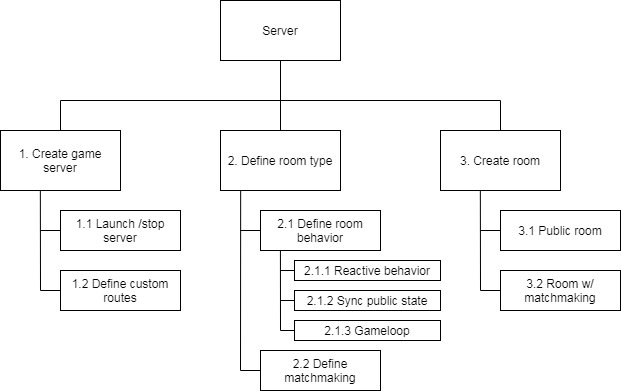
\includegraphics[scale=0.5]{images/2-scoping/server-RBS.png}
   \centering  
   \caption{\textit{RBS for srrver side user requirements.}}
  \label{fig:server-RBS}
\end{figure}

\begin{figure}[H]
  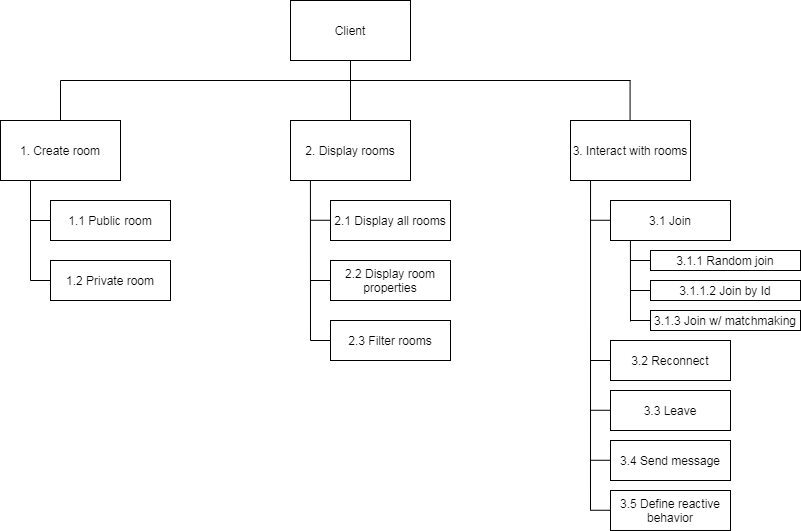
\includegraphics[scale=0.5]{images/2-scoping/client-RBS.png}
   \centering  
   \caption{\textit{RBS for client side user requirements.}}
  \label{fig:client-RBS}
\end{figure}
 
\subsubsection{Use Cases}

We can split use cases in two scenarios about role played by clients: clients that joined a room and clients that didn't. In the first case, the whole system is the context, and it explains high level functionalities of the system. In the latter case, the context is the interaction between a client in a room and such room.

\bigskip
Starting from the first scenery, we have client side and server side programmers that make use of the library as entities interacting with the system.
\\
This is shown in UML use case diagram in figure \ref{fig:system-use_cases}.
\begin{figure}[H]
  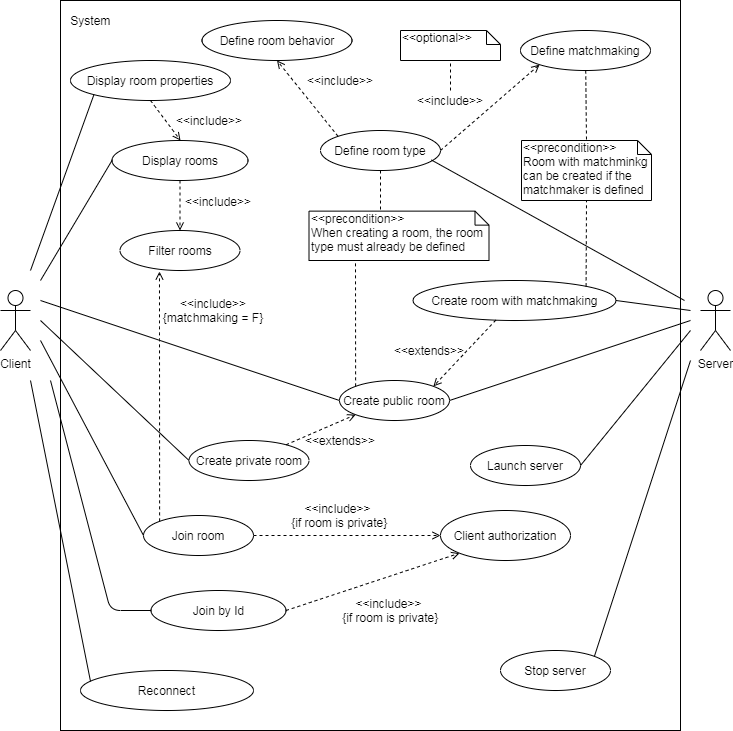
\includegraphics[scale=0.5]{images/2-scoping/system-use_cases.png}
   \centering  
   \caption{\textit{Use case diagram of the system.}}
  \label{fig:system-use_cases}
\end{figure}

\bigskip
About joined room interaction, interacting entities are client side programmer as before for clients, and, a room agent for server, intended as the server side programmer (as before) and/or the room itself with its reactive/proactive behavior defined by the programmer. 
\\
This is shown in UML use case diagram in figure \ref{fig:room-use_cases}.
\begin{figure}[H]
  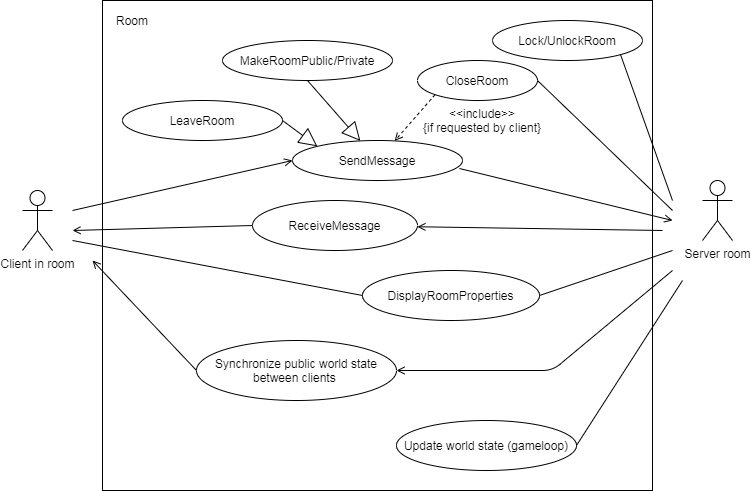
\includegraphics[scale=0.5]{images/2-scoping/room-use_cases.png}
   \centering  
   \caption{\textit{Use case diagram about room interaction scope.}}
  \label{fig:room-use_cases}
\end{figure} 
 
\subsection{Functional Requirements}

Functional requirements, i.e. capabilities that the system should provide, are expressed in table \ref{table:server-f-req} and \ref{table:client-f-req} for server and client respectively.

\begin{center}
  \begin{longtable}{|l|l|} 
    \caption{\textit{Server functional requirements.}} \label{table:server-f-req} \\
  
\hline
ID   &  Specification \\
\hline
\multicolumn{2}{|c|}{} \\
\hline
1         & Create and handle game server \\
1.1       & Launch game server on provided address and port \\
1.2       & Define behavior on server start up \\
1.2       & Suspend/terminate server \\
1.4       & Define behavior on server stop \\
1.5       & Resume suspended server \\
1.6       & Accept user defined routes \\
2         & Define room type \\
2.1       & Define room behavior \\
2.1.1     & Define room reactive behavior \\
2.1.1.1   & Define on create behavior \\
2.1.1.2   & Define on join behavior \\
2.1.1.3   & Define on message received behavior \\
2.1.1.4   & Define on leave behavior \\
2.1.1.5   & Define on close behavior \\
2.1.2     & Define room proactive behavior \\
2.1.2.1   & Handle public state synchronization between clients \\
2.1.2.1.1 & Start state synchronization between clients \\
2.1.2.1.2 & Stop state synchronization between clients \\
2.1.2.1.3 & Resume state synchronization between clients \\
2.1.2.1.4 & Set state synchronization rate\\
2.1.2.2   & Handle room state periodic update (gameloop)  \\ 
2.1.2.2.1 & Start room state periodic update (gameloop) \\
2.1.2.2.2 & Stop room state periodic update (gameloop) \\
2.1.2.2.3 & Resume room state periodic update (gameloop) \\
2.1.2.2.4 & Set state update rate (gameloop) \\
2.2       & Define room properties\\
2.2.1     & Public/private property should be given by default \\
2.2.2     & Room property types could be int, string, boolean, double \\ 
2.3       & Define room state \\
2.4       & Define room type matchmaker \\
2.5       & Ignore multiple room type definitions from second on \\
2.6       & Define custom join constraints depending on room type \\
3         & Lock/unlock room \\
3.1       & Rooms are unlocked by default \\
4         & Close room \\
4.1       & Directly close the room from server \\
4.2       & Expose possibility to close a room for clients \\
4.3       & Notify a client that the room has been closed \\
4.4       & Room auto closing \\
4.4.1     & Allow room auto closing \\
4.4.2     & Auto closing is off by default \\
4.4.3     & Close as auto close timeout expires \\
4.4.4     & Close in front of direct close request even if auto close is on \\
5         & Create room \\
5.1       & Create public room \\
5.2       & Create room with matchmaking \\
5.2.1     & Room with matchmaking should define clients allowed to join \\
5.3       & Rooms create be the server should contain no client at the beginning \\
6        & Display room properties \\
7        & Send messages to clients in a room \\
7.1      & Send a message to one specific client (tell) \\
7.2      & Send a same message to all clients in the room (broadcast) \\
8        & Monitor client liveness \\
8.1      & Heartbeat service (if activated) \\
8.2      & Inactive clients kicking on timeout (if activated) \\
9        & Deny join to room under certain circumstances \\
9.1      & Deny join to private room if no correct password is provided \\
9.2      & Deny join to a locked room \\
9.3      & Deny join to closed room \\
9.4      & Deny join to matchmaking room if not in expected players \\
10        & Allow reconnection for clients to a room \\
10.1      & Allow configuration of a reconnection period length \\
10.2      & Fail reconnection to room under certain circumstances \\
10.2.1    & Fail reconnection to room if client din't previously join the room \\
10.2.2    & Fail reconnection to room if it took too long for the client to reconnect \\
10.2.3    & Reconnection feature is disable by default \\
10.2.3.1  & Allow reconnection timeout length configuration when enabling such feature \\
10.3      & Reconnetion is not considered as a join event \\
11        & Expose possibility to create rooms for clients \\
11.1      & Expose possibility to create public rooms for clients \\
11.2      & Expose possibility to create private rooms for clients \\
12        & Expose possibility to make room public/private for clients \\
\hline

  \end{longtable}
\end{center}

\begin{center}
  \begin{longtable}{|l|l|} 
    \caption{\textit{Client functional requirements.}} \label{table:client-f-req} \\
 
\hline
ID   &  Specification \\
\hline
\multicolumn{2}{|c|}{} \\
\hline
1       & Display all rooms of a given type, private and public both \\
1.1     & Locked rooms should not be displayed \\
1.2     & Matchkaing room should not be displayed \\
1.3     & Rooms can be filtered on their properties \\
1.4     & Room Ids should be visible to clients \\
1.3.1   & Allowed filter straegies are equal, not equal, grater, lower \\
2       & Display all joined rooms, locked and with matchmaking too \\
2       & Create a room \\
2.1     & Create a public room \\
2.2     & Create a private room \\
2.3     & Fail on  create the room if its type is not already defined server side \\
2.4     & Define starting room properties values \\
2.4.1   & Ignore a given room property if such property is not defined in the room \\
3       & Join room \\
3.1     & Join without matchmaking \\
3.1.1   & Random join to public room \\
3.1.1.1 & Allow to specify filters on joinable rooms \\
3.1.2   & Join by room Id \\
3.1.2.1 & When joining by ID, give possibility to provide a password \\
3.1.2.2 & When joining by ID, a provided password will be ignored if the room is public \\
3.1.3   & Auto join a room when creating such room \\
3.2     & Join with matchmaking \\
3.2.1   & Join by Id is not allowed \\
3.2.2   & Filters on rooms with mathcmaking is not allowed \\
4       & Leave a room \\
4.1     & Leaving a room is allowed only if such room has been previously joined \\
5       & Reconnect to room \\
6       & Visualize room properties \\
6.1     & Visualize all properties in a room \\
6.2     & Retrieve value of a single property \\
6.2.1   & Notify error if the specified property does not exist \\
7       & Send messages to a room \\
7.1     & Sending messages to room is enabled once the client joined the room \\
7.2     & When sending amessage to a room, no reply is expected \\
8       & Define reactive behavior to room events \\
8.1     & Define behavior on received message from the room \\
8.2     & Define behavior on state update \\
8.3     & Deifne behavior on room closing \\
8.4     & Definition of reactive behavior is allowed once the client joined the room \\
9       & Close a room \\
11      & Change public/private state of a room \\
11.1    & Make a public room private \\
11.1.1  & When making a public room private, the provision of a password is mandatory \\ 
11.2    & Make a private room public \\
\hline

  \end{longtable}
\end{center}

\newpage

\subsection{Non functional Requirements} 

\begin{itemize}
	\item[\emph{Usability}] The provided library should be easy to use by game developers that are unfamiliar with client-server interaction and newtwork communication protocols.
	\item[\em{Portability}] The provided library should be used in both server and client environments on all major operating systems (i.e Windows, Linux and MacOS).
\end{itemize}


TODO
- deployment 


\subsection{Implementation Requirements}
The library must be implemented using Scala as programming language.
  
 
 

 
\chapter{Development process}

The chosen project management lifecycle (PMLC) is an agile one, in particular Scrum. 
\section{Interactions planning}

In order to end within the given deadline of 50 days, a total of 7 sprints is scheduled. Each sprint is planned to last one week, from Sunday to Sunday.
\\
As Scrum process suggests, each sprint is provided with an initial planning phase and is concluded with review and retrospective meetings. Both current sprint closing and next sprint planning are supposed to be done on Sunday.
\\
Moreover, daily scrum would often be required when tricky features are realized or any non negligible issue is found. Obviously, informal quick message exchange is allowed between team members all day long.
\\
The only exception to such organization is given by the first sprint. Indeed, requirement analysis and system design are predominantly realized at this time, and daily meetings are required to achieve these tasks so that the product backlog, required to plan each sprint from the second on, is produced.
\\
During all the phases of the development process software like Trello and Microsoft Teams are used to support team interaction.


\section{Tasks split and assignment}

Once the product backlog is available, each sprint planning phase produces a sprint backlog containing tasks to complete before such sprint ends. Tasks are chosen from product backlog by priority (importance of a feature in term of business value), considering the estimated size of each task too, so that no sprint is excessively weighted down. Once a task is selected from product backlog, it is split in subtasks by detailing its aspects. Tasks and subtasks size is expressed using Fibonacci sequence. 
\\
Once the spint backlog is built, starting tasks are agreed between all team members, and each one takes charge of a couple of them (2-3 approximatively). The remaining ones are assigned day by day, looking to how the development proceeds. There is no general a priori criteria for task assignment; the only aspect considered, when possible, is to minimize the dependency between tasks assigned to different team members. 
\\
During sprint review, individual work of each member is examined to understand the current situation and to realize if any improvement is needed.

\section{Development tools: Build, Testing, CI}

The building system is automated using the sbt build tool since it is well integrated with Scala.
\\
The development process is not strictly a TDD approach but unit tests on single components and integration tests on use case scenarios are provided to ensure system correctness.  
\\
Moreover,``TravisCI'' combined with ``Github'', is used as continuous integration tool to perform regression tests. Repository is handled with pull requests reviewing flow.
\\
In the end, another plugin/tool used would be ``scalastyle'' in order to check code style adherence to specified conventions.

\subsection{Ensure system portability}

By looking to non functional requirements, portability comes out to be a key aspect. In order to ensure this requirement, Travis is configured to build and test the library upon multiple platforms and OS. In particular:
\begin{itemize}
\item \textbf{OS\footnote{Scala integration with Windows in not available on Travis yet}}: 
  \begin{itemize}
  \item \textit{Linux}
  \item \textit{Osx (MacOS)}
  \end{itemize}
\item \textbf{JDK}:
  \begin{itemize}
  \item \textit{openjdk11}
  \item \textit{openjdk13}
  \item \textit{openjdk-ea (early access)}
  \end{itemize} 
\end{itemize}  











 
\chapter{System architecture}
Since the library is based on the client-server architectural pattern, its functionalities are split in two distinct modules: 
\begin{itemize}
	\item \textit{Client module} - It provides the features required to connect and communicate with a game server. In particular, it allows the client side developer to create rooms (that will be hosted on the server) and to perform operations on them (e.g. join, leave, message...).
	\item \textit{Server module} - It internally implements the logic to handle clients connections and it allows the developer to run a gameserver and to define new types of room. Moreover, it contains all the logic to handle matchmaking requests too.
\end{itemize}

Client and server modules are not fully separated but, on the contrary, they share some common concepts like communication protocol and data serialization utilities required when parsing data received and sent through the network.
\\
A common notion of room is the most important concept that clients and server must agree to. That is decribed in section \ref{room-arch}. 

\section{Room} \label{room-arch}


\begin{figure}[H]
	\centering
	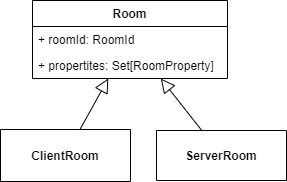
\includegraphics[scale=0.7]{images/3-architecture/room-class-3.png}
	\caption{Room class diagram}
	\label{fig:room_classes}
\end{figure}


At the most abstract level, a room is an entity that owns an unique Id and some properties that describe the room itself (figure \ref{fig:room_classes}).
\\
This is the basic model shared beween clients and server that each model will extend.

\bigskip
\textit{ServerRoom}
\\
The server room is the one that will be used by the server side developer. It provides functionalities to communicate and interact with connected clients. Besides, as specified in server requirement 2.1, the room behavior can be defined by the developer according to the application custom logic.

\bigskip
\textit{ClientRoom}
\\
On the other hand, the client room is the room that a client side developer will use. This component is meant to provide an interface towards the server side room, so that the developer can both send and receive messages from it. Obsviously, it exposes functionalities to define custom behavior too, as specified in client requirement 9.

\section{Server architecture} \label{sec:server_arch}
The main components of the server side architecture are visible in figure \ref{fig:server_classes}. 

\begin{figure}[H]
	\centering
	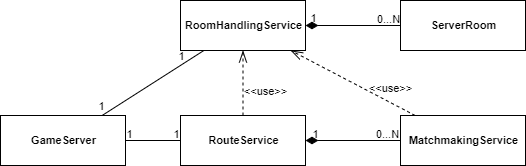
\includegraphics[scale=0.7]{images/3-architecture/server-architecture.png}
	\caption{Server architecture}
	\label{fig:server_classes}
\end{figure}

\bigskip
\textit{GameServer}
\\
The GameServer is the main component of the architecture. It is the one that listen and handle client connections and is also the starting point from where all the other components are created.

A developer will mostly use the server module of the library working with the interface that this component exposes.

As shown in figure \ref{fig:server_classes} it is connected with two other classes that are the RouteService and the RoomHandlingService.

\bigskip
\textit{RoomHandlingService}
\\
As the name suggests, the RoomHandler is the component used to manage rooms. It is meant to: 
\begin{itemize}
	\item Keep track of which rooms are currently active in the system providing a way to interact with them (e.g create new ones or delete existing)
	\item Provide a way to define new type of rooms that, upon a specific client requests, will be created.
\end{itemize}

\bigskip
\textit{RouteService}
\\
Defines the routes that the clients should use to interact with the server and implements all the handlers associated with them. A client request received by the gameserver is indeed served by this component. 

Client requests can basically be split in two types:
\begin{itemize}
	\item requests concerning rooms (e.g connect to a room or retrieve available rooms...)
	\item requests concerning matchmaking (e.g join a matchmaking queue)
\end{itemize}
This component uses a RoomHandler to manage the first type and a list of MatchamkingServices (one for each type of room defined by the user) for the second type. 

\bigskip
\textit{MatchmakingService}
\\
The MatchmakingService is the component that implement the matchmaking logic for a given type of room (i.e. adding clients to a queue and eventually create groups according to some information on those clients). It also needs to use a RoomHandler since, when the a group of client is formed, a room where this clients will connect must be created.



\section{Client Architecture}

\begin{figure}[H]
	\centering
	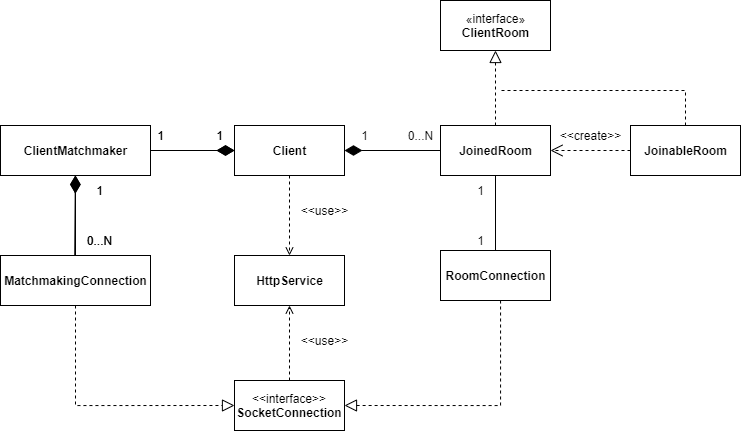
\includegraphics[scale=0.65]{images/3-architecture/client-architecture.png}
	\caption{Client architecture diagram}
	\label{fig:client_architecture}
\end{figure}

\section{Client-Server Interaction}
The requirements analysis led to the definition of three types of interaction between client and server:
\begin{enumerate}
	\item Client to GameServer \\
	This interaction takes place in those situations where the client makes a request to the server and waits for a specific response: for example getting the list of all rooms that can be joined. We decided to handle this kind of requests defining a REST protocol as shown in table
	 \ref{table:server_routes}.
	\begin{table}[]
		\begin{tabular}{p{2cm}p{4cm}p{2cm}p{5.5cm}}
			\textbf{Http Method} & \textbf{Path}	  & \textbf{Payload}  & \textbf{Result}                                                            		\\\\
			GET                  & /rooms             & filters           & get all the rooms that match the filters in the payload                        	\\\\
			GET                  & /rooms/:type       & filters           & get all the rooms with the given type (filtered by filters in the payload)     	\\\\
			GET                  & /rooms/:type/:id   & empty             & get the room with the given id searching among rooms of the given type         	\\\\
			POST                 & /rooms/:type       & options           & create a room of the given type with the option passed in the payload          	\\\\
			GET                  & /connection/:id    & websocket request & open a web socket connection with the room that has the given id               	\\\\
			GET                  & /matchmaking/:type & websocket request & open a web socket with the matchmaking service relative to the given room type 	\\\\
		\end{tabular}
		\caption{\label{table:server_routes} \textit{Server REST protocol for request-response interaction}}
	\end{table}
	\item  Client to Room \\
	In this case we are in a situation where a client wants to establish a connection with a given a room to both send and receive messages from it. The request-response pattern doesn't work here because now the communication channel must be full-duplex: the server can send data to the client even without a specific client request (for example if the room broadcasts a message to all connected clients).
	
	The chosen solution here is the websockets protocol since it provides the exact described behavior. Specifically, when a client wants to interact with a room, a websocket between that client and the server is created; the messages that the client sends through the socket are redirected to the room and the messages that the room wants to send to that client are forwarded through the socket. 
	
	Another consideration to make here is that clients can receive and send different types of messages through the socket: first of all they need to send a join message to notify the room that they want to enter; then they may want to send generic messages to that room (e.g. actions that affect the current game state) and eventually they'll want to leave the room, and so on \dots
	In order to identify this different kind of messages we decided to define a communication protocol that is used for messages in the websocket.
	
	
	\item Client to Matchmaking \\
	The last type of interaction is the one that takes place when a client wants to join the matchmaking queue for a given type of room. In this case the client asks the server to be added to the queue and waits to be grouped with other clients. We have decided to use websockets here too since when the client sends the request, the server response is not immediate. The communication must be kept open until the matchmaking service doesn't create the group of client to start the match. Only then the server can respond to the client with a message that contains the information to join the room that will host the game.
\end{enumerate}










\chapter{Detailed design}

\section{Actor model}

In each module we can detect few different components that may interact in a very complex way. Moreover, each component may own more than one control flow. This could lead to a growth in design complexity and to potential concurrency issues to be solved.
\\
In order to cut those aspects down, components are organized using an actor model. This way, components can be seen as self-contained services that communicate using message passing.
\\
The only drawback is the exposure of the actor model to users that may be forced to think in term of a non trivial programming paradigm. In order to prevent that, library logic and structure is hidden behind an interface layer. This can be achieved just by using a simple facade pattern that permits to mask actor model and message passing by using the solely asynchronous programming, simpler to users the may not know the actor model and more general for users that wouldn't structure their programs using actors.

\section{Rooms}

\subsection{ServerRoom}
\begin{figure}[H]
	\centering
	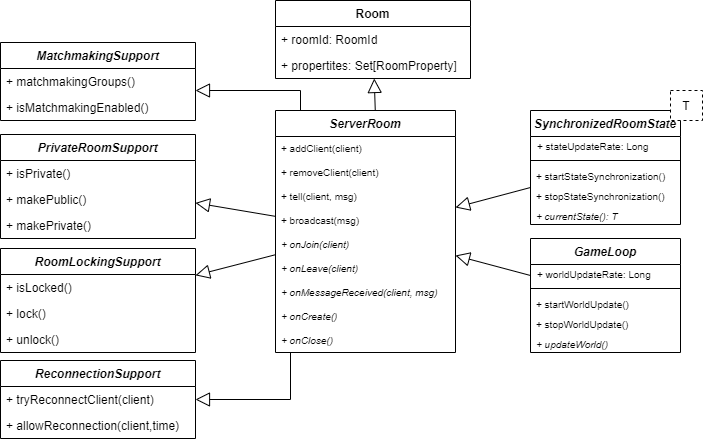
\includegraphics[scale=0.5]{images/4-design/server-room.png}
	\caption{Server room class diagram}
	\label{fig:server_room_class_diagram}
\end{figure}
\texttt{ServerRoom} is a trait that encapsulate the concept of room used server-side; as we see in figure \ref{fig:server_room_class_diagram} it extends the \texttt{Room} trait adding methods to manage clients (add,remove, tell and broadcast) and defining abstract handlers for room events. These handlers are the ones that the developer must implement to define his own type of rooms.

Since the developer may also want to automatically synchronize the state of the game and have an inner game loop (requirements 2.1.2.1 and 2.1.2.2), there are two extension of the server room: \texttt{SynchronizedRoomState} and \texttt{GameLoop} that provide this functionalities. 

The first one is a trait generic in the type of the state that needs to be synchronized to clients; this trait has all methods implemented except for \texttt{currentState} that must be defined by the user and will be called periodically at the specified rate: \texttt{stateUpdateRate}.

The second one, \texttt{Gameloop}, is also a trait but is not generic and requires to define \texttt{updateWorld}, a void method that will be called every \texttt{worldUpdateRate} milliseconds.

While this two traits can be optionally mixed in a ServerRoom, all those that in figure \ref{fig:server_room_class_diagram} are shown on the left, are functionalities that a room has by default:
\begin{itemize}
	\item \texttt{MatchmakingSupport}: gives the developer access to the matchmaking groups that the matchmaking service associated with this room has created.
	\item \texttt{ProvateRoomSupport}: used to set a password to the room in order to prevent access to some clients.
	\item \texttt{RoomLockingSupport}: enables lock and unlock functionalities to the room. 
	\item \texttt{ReconnectionSupport}: allows clients to reconnect to the room within a certain period of time.
\end{itemize}

\subsection{ClientRoom}

\subsection{Properties and Filters}

UML class diagram in figure \ref{fig:property-class} shows the detailed architecture of room properties and filters.

\bigskip
\textit{Basic room properties}
\\
Each property (\texttt{BasicRoomProperty}) owns a name and a value.
\\
Values, since they can be of four types (server requirements 2.2.2), are modelled as classes that extend a common trait \texttt{RoomPropertyValue}. This trait wraps a ``real'' value of type \texttt{Int}, \texttt{Double}, \texttt{Boolean} or \texttt{String}.
\\
Each property value exposes two main feaures: the real value wrapped by the class and a method that compares such value to another one of the same type (e.g. compare the Int value wrapped by the class to another given Int); this is useful since different type of values may define different comparing logics.
Moreover, there is also a static factory that permits to create a property value from a given first class value (if possible).

\bigskip
\textit{Filters}
\\
By looking to client requirement 1.6.1, there are four available filter strategies. Similarly to property values, they are hidden behind a common trait \texttt{FilterStrategy}. Such trait defines a name for the strategy and an evaluation predicate that permits to apply the strategy to two values. The evaluation result expresses if the filtering defined by the strategy is satisfied.

\bigskip
Since library usability is a core aspect, a simple DSL language is created in order to easily manage filters.
\\
\texttt{BasicRoomProperty} functionalities are extended to include filters by using mixins. This way, filter strategies can be directly called by the property itself.
\\
A \texttt{FilterOption} is something that contains the name of the property to be filtered, the strategy to be uses and a value the property should be compared to. It exposes an utility method to concatenate two \texttt{FilterOption} too.
\\
A \texttt{FilterOptions} is a wrapper around a set of \texttt{FilterOption}; this is useful when talking about DSL since it permits to define static factories (\texttt{empty}, \texttt{just}) and utility methods such as concatenation (\texttt{and}) and union (\texttt{++}).

\bigskip
\textit{Design notes / implementation directives}
\\
\begin{itemize}
\item Before on choosing this desing, few different options have been analyzed, and this has been decided to be the most feasible one. The only lack that can be detected is on the value getter of \texttt{RoomPropertyValue}. Indeed, it is absent in the class instance itself, and it is only available through the static method \texttt{valueOf}.
\item Notice that, in order to encourage library usability, the value wrapper can be made be transparent to final users thanks to implicit conversions that can be defined in Scala.
\end{itemize}

\begin{figure}[h]
	\hspace*{-0.1in}
	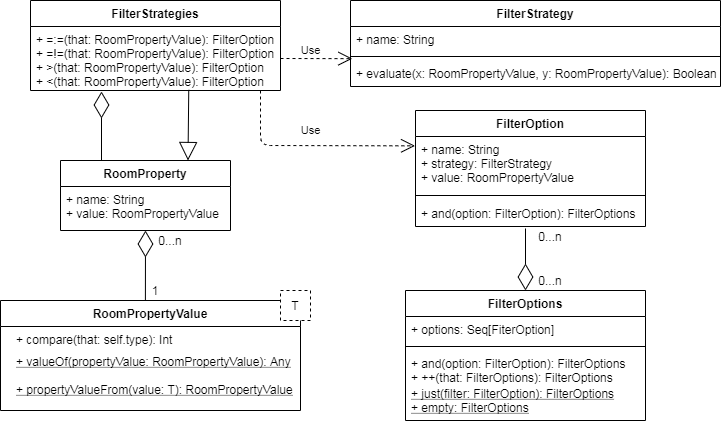
\includegraphics[scale=0.55]{images/4-design/property_and_filters-class.png}
	\caption{Properties and filters class diagram.}
	\label{fig:property-class}
\end{figure}


\section{Server}
Class diagram in figure \ref{fig:server_class_diagram} describes in detail the server architecture displaying the main functionalities of the classes and showing how actors interact with all the other components. 
\begin{figure}[h]
	\hspace*{-1.1in}
	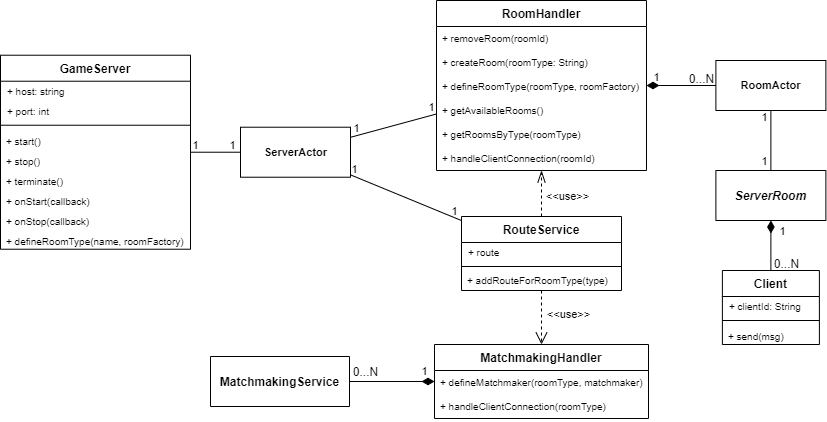
\includegraphics[scale=0.55]{images/4-design/server_class.png}
	\caption{Server class diagram}
	\label{fig:server_class_diagram}
\end{figure}

The \texttt{GameServer} class is the facade interface that is exposed to the developer. It internally creates a \texttt{ServerActor} that is the entity that acts as the real server listening for clients requests. This actor creates a \texttt{RouteService} object that is used to know which routes to use and how to handle requests; it also allows to dynamically define new room types that will be used by te server. 

The \texttt{ServerActor} also uses a \texttt{RoomHandlingService} actor to create and define rooms from the server. The same actor is used by the RouteService.

As we described for the server architecture in section \ref{sec:server_arch}, the purpose of the \texttt{RoomHandlingService} is to manage the active rooms in the applications. Specifically though it doesn't directly create rooms but instead it creates \texttt{RoomActors}: actors used as 'wrappers' for ServerRooms to avoid concurrency issues; more than one client can indeed interact with a single room at the same time, so, in order to avoid race coditions, we decided to make clients communicate with RoomActors that process messages sequentially. Each actor is in charge of notifying clients' actions to the room that is associated with.

Each \texttt{ServerRoom} is linked to an actor and keeps track of connected clients (\texttt{Client} class in figure). Clients are uniquely identified by their id and expose a \texttt{send} method that allows to send messages to them. It is important to notice that each room has its own view of clients: the same client connected to different rooms will have a different id in each of them. 

Clients are also used by the \texttt{MatchmakingService} since is the actor that performs matchmaking operations and needs to know which clients are waiting to start a match. \texttt{MatchmakingService} actors are spawned during server startup if the developer used the \texttt{defineRoomWithMatchmaking} method to define a room. 

Since clients can make requests for matchmaking, the \texttt{RouteService} use a \texttt{MatchmakingHandler} to redirect those requests to the right \texttt{MatchmakingService} actor.


\section{Client}

\begin{figure}[H]
	\hspace*{-1.7in}
	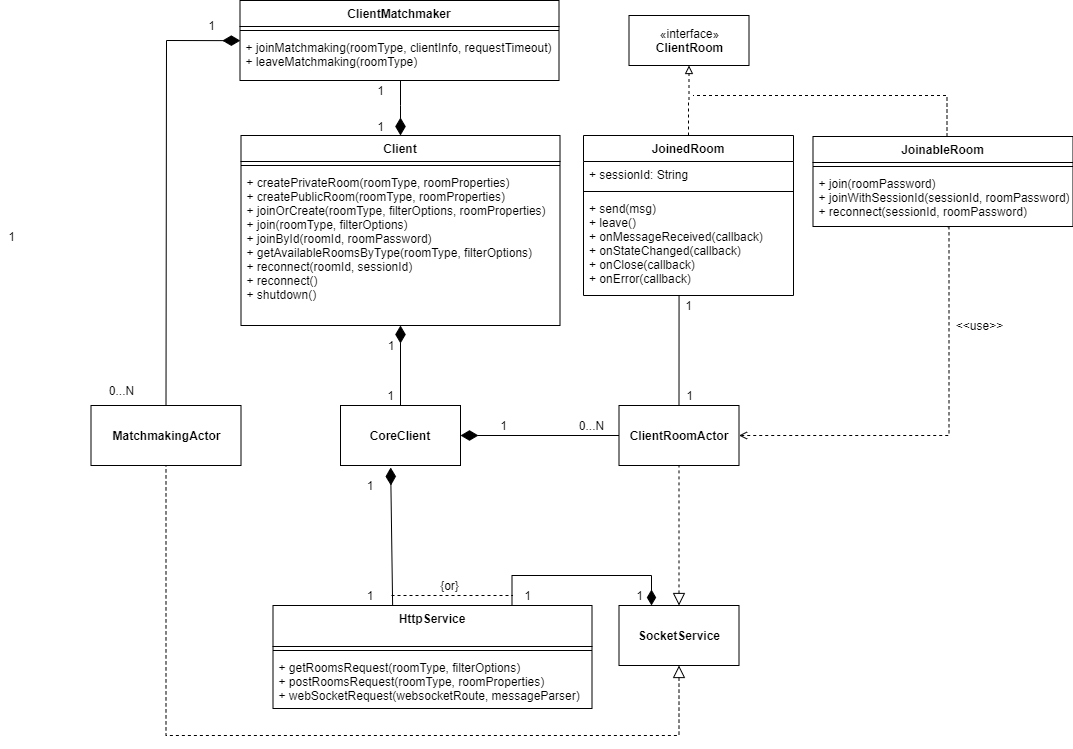
\includegraphics[scale=0.55]{images/4-design/client_class.png}
	\caption{Client class diagram}
	\label{fig:client_class_diagram}
\end{figure}

\section{Communication}\label{sec:communication_design}


\subsection{Json Serialization}
For Request-Response interaction (described in section 3.4), we decided to use json format for both client requests and server responses. We have defined a class that provides json-formatted serialization capabilities for all entities that are exchanged at this stage of client-server interaction that are specifically:
\begin{itemize}
	\item SharedRoom objects
	\item Room properties
	\item Room filters
\end{itemize}

\subsection{Websockets}
\begin{figure}[h]
	\hspace*{-0.5in}
	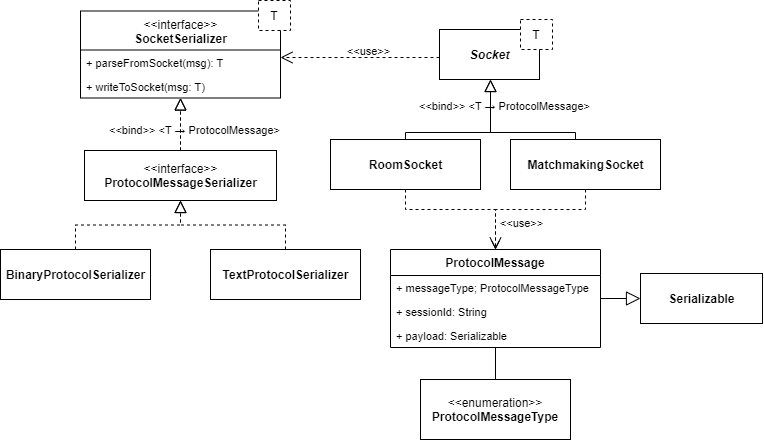
\includegraphics[scale=0.6]{images/4-design/communication_protocol.png}
	\caption{Websocket class diagram}
	\label{fig:websocket_communication_design}
\end{figure}
Regarding websockets instead, the design is more structured. A class diagram describing the main classes is shown in figure \ref{fig:websocket_communication_design}.
The \texttt{Socket} abstract class provides the main functionalities for a socket communication and allows to define the configurations for the connection: heartbeat rate and idle timeout. It is generic in T where T represents the type of messages sent through that socket . Two concrete implementations are provided for this class:
\begin{itemize}
	\item \texttt{RoomSocket}: used for the communication between client and rooms.
	\item \texttt{MatchmakingSocket}: used for the communication between client and matchmaking servicess
\end{itemize}
They both are Socket where the generic type T is a \texttt{ProtocolMessage}. This is indeed the class that defines the communication protocol between client and server. It has 3 fields to describe a message sent through a socket:
\begin{itemize}
	\item \textit{messageType} \\
	Used to identify the type of message that the client or the server want to send. The list of the possible message types is defined in the ProtocolMessageType enumeration.
	\item \textit{sessionId} \\
	This is used to identify the client that is sending the message through the socket. When a websocket connection is established between client and server, a unique id is genereated; the client must always uses the same sessionId to send messages through that socket.
	\item \textit{payload} \\ 
	An optional payload that can be carried with the massage. This is for example the field that is set when the developer use the 'sendMessage' method on the client room. It must be Serializable since it will eventually be serialized to be sent to the server.
\end{itemize}

In order for a Socket object to send and receive data, it must be able to serialize and deserialize the messages that pass through it. It uses for this purpose a \texttt{SocketSerializer} that has two methods: parsefromSocket and writeToSocket. This class is also generic in T that is the type of messages that needs to read and write.

Since \texttt{RoomSocket} and \texttt{MatchmakingSocket} needs to handle \texttt{ProtocolMessage}s we defined a \texttt{ProtocolMessageSerializer} interface that specifically defines a serializer for protocol messages. We implemented two types of serializers: \texttt{BinaryProtoclSerializer} and \texttt{TextProtocolSerializer}. The first one serialize protocol messages as binary data; the latter instead as text messages.
 
We have two different implementations because we initially thought to use Json also for socket communication and this would be done by the \texttt{TextProtocolSerializer}. However, we eventually decided to use binary representation both to improve performance and usability, so we switched to the \texttt{BinaryProtocolSerializer}.


An example of a full interaction between client and server is shown in the sequence diagram in figure \ref{fig:create_room_seq}
\begin{figure}
	\hspace*{-1in}
	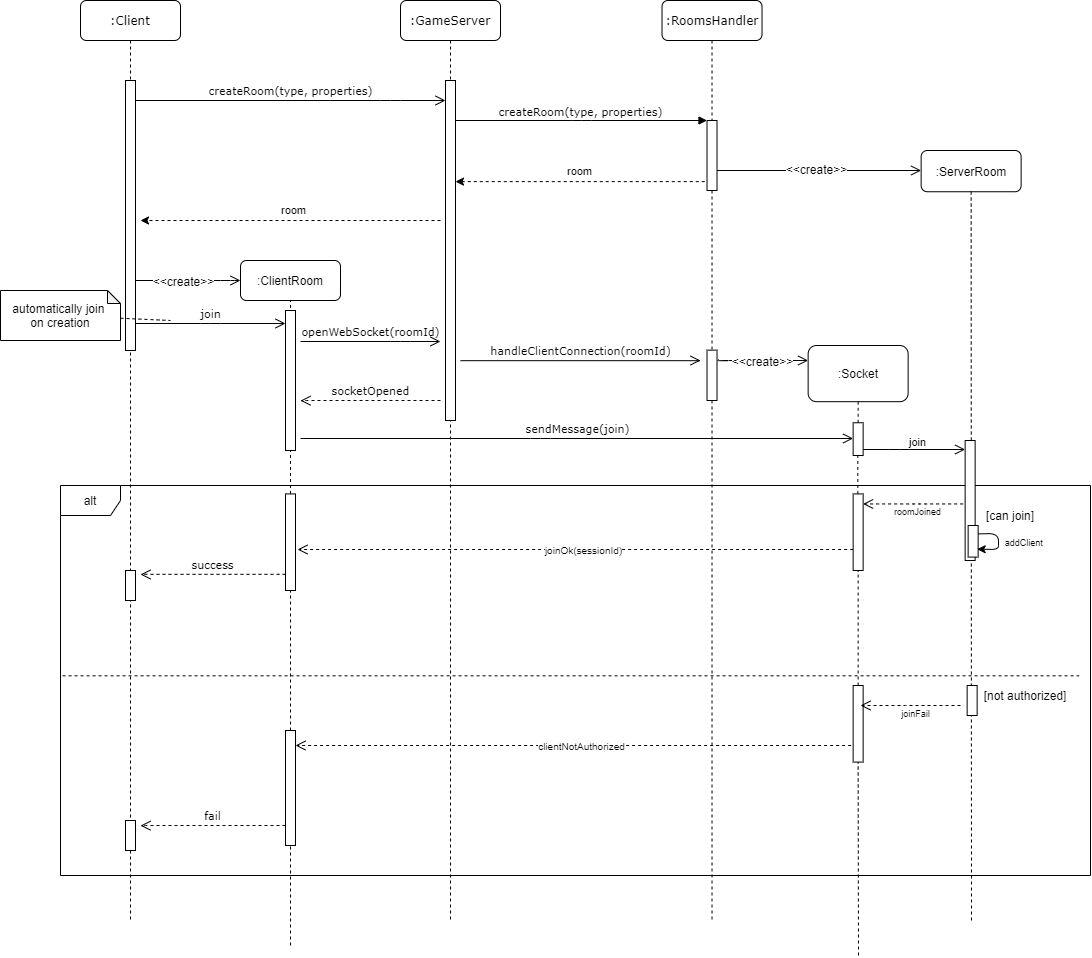
\includegraphics[scale=0.5]{images/4-design/create_room_seq.png}
	\caption{Example of a client-server interaction upon a 'create room' request}
	\label{fig:create_room_seq}
\end{figure}
\input{5-implementation.tex}
\chapter{Retrospective}

\section{Development description in detail}

\subsection{Sprint 0}
\subsubsection{Report}
Product backlog was defined during first meetings. Each item in the backlog was associated to an estimate of his development effort.
\\
The organizational structure of the project was defined too. We discussed tools and development environments to support continuous integration.
\\
Initial analysis and design process were performed in order to define main entities of the system and their interactions.
Therefore, it was decided to internally use an approach base on actors, which however would have been transparent to the final user (developer). This is due to an elevated complexity of the system, and an actor model could simplify few aspects. 
We decided to rely upon ``akka-core library'' and ``akka-http library''. 
\\
In the end, it was decided to carry out client and server modules development in parallel in order to have a working core in the shortest time. This core would be extended incrementally during the project lifetime.




\subsection{Sprint 1}
\subsubsection{Report}
The goal of this first sprint was to define main client and server interfaces and to set up a minimal working system that allows:
\begin{itemize}
	\item Game server execution 
	\item Room types definition
	\item Handling of client requests to create rooms.
\end{itemize}
These goals were completed successfully. 
\\
An issue regarding the extension of an already existing server was found due to internal ``Akka'' policies. 
This ended up in a revision on some decisions that were made about server creation. The result is that it is possible for the user to specify external routes which will be handled by the game server (if they don't conflict with the already existing ones internally used  by the game server itself). 
However, it is not possible to attach the game server to an existing one.
\\
However, even if in a different way than the one prospected at the beginning, the requirement can be considered fulfilled.   




\subsubsection{Retrospective}
The task effort concerning the creation of a game server based on an existing one was underestimated, and it created few troubles during the whole week.
\\
The team was able to complete all tasks and effectively use continuous integration and project management tools decided during first meetings.
\\
A problem that arose was that some ``scalastyle'' rules were too strict, and tests were failing for no good reasons. We decided then to disable such rules for further development.


\subsection{Sprint 2}
\subsubsection{Report}

During this week some of the main features of the library about clients and rooms have been developed.
\\
Tasks regarding web socket support was underestimated, and it was not fully completed during this sprint.
The interaction between clients and rooms required the definition of an ad hoc protocol to manage messages internally used by the library. This introduced some dependencies between client and server tasks causing little slowdown in the development process.
\\
Given the amount of work spent on such task, some others were left behind and not fully achieved too (e.g. the creation of rooms with custom options).
\\
Uncompleted tasks will be completed in the next sprint.



\subsubsection{Retrospective}
Even if the amount of work spent on this sprint was certainly greater than the previous one, the fact that the team was not able to complete all tasks requires some further considerations.
\\
It's important to better define the work in advance. For example, we should consider splitting tricky tasks in multiple sub-tasks when needed, so that hidden dependencies are found and parallel work can be easily planned and carried out.
\\
The creation of rooms with custom options was not completed due to the lack of communication about who was the volunteer of such task, and, in the end, we run out of time.
\\
Furthermore, team communication should be increased during the week.
This could help by solving in advance problems that arise during development.

\subsection{Sprint 3}
\subsubsection{Report}

In this week, pending tasks from previous sprint were completed.

While implementing automatic state update, we decided to use binary serialization instead of Json one. The latter required the user to define his own parsers while binary serialization allowed a more generic and simple approach.

Since the work done in the previous weeks contained the core features of the library, we were able to implement a first simple example of online multiplayer game: ``Rock-Paper-Scissor''. 
The main purpose was to verify effective usability of features produced so far, both for client and server sides.
The final code is also a good explanation about how to use the library and its basic functionalities.


\subsubsection{Retrospective}
Tasks were all completed this time; anyway, the lack of documentation and diagrams relative to some common concepts led to few integration issues on code produced by different team members. Sometimes, ad hoc refactoring was needed to keep high software quality throughout the development.
\\
Increased care must be granted to future documentation process.
\\
During the week, few unpredictable tests were added to the test suite.
As they were found, they were immediately fixed within the end of the sprint.




\subsection{Sprint 4}
\subsubsection{Report}
In this sprint, other main features were added, such as game loop on server rooms and client re-connection.
\\
Moreover, it was implemented ``MoneyGrabber'', a second game that takes advantage of more advanced features of the library, such as the automatic state update and the management of rooms with multiple players.
Therefore, it was possible to verify the actual versatility of the library showing a further and more complex example of use in a real context.
\\
All tasks were completed ahead of time.
\\
In the end, a first closing process, that is the sistematic writing of the report by using gathered informal notes and documentation, has been started.

\subsubsection{Retrospective}

During this sprint the team worked very well, probably helped by the solid core already implemented that was easily extensible.
\\
Probably, we should have considered the addition of some more tasks to the backlog in the sprint planning.
\\
By the way, the remaining time of the sprint was used by the whole team to improve the existing code quality and to produce some more detailed documentation.
\\
The only drawback was the underrate of game loop consequences on the whole system. Indeed, game loop, and also the already implemented state synchronization feature, might imperil system safety due to possible concurrency problems. A meeting with the team was required to improve some design aspects so it was possible to solve any issue while keeping it transparent to final user; it took a non negligible amount of time.

\subsection{Sprint 5}
\subsubsection{Report}
\subsubsection{Report}
Matchmaking functionality was implemented during this sprint.
A revise on client-server communication protocol was required to integrate matchmaking service in the system.

\subsubsection{Retrospective}

Given the importance of the new matchmaking feature, we decided to develop a further example showing its use in an example application. This will be done in the next sprint.
\\
The revision of communication protocol was due to some non trivial matchmaking aspects that were non fully considered in advance, such as data flows and separation between normal and matchmaking rooms. 
\\
In the end, we noticed that client-side room closure feature was not explicitly defined yet. 
After a brief discussion, we decided that a developer could implement such functionality by using existing features (e.g auto-close feature on server-side) in a safer and robust manner. Hence, we considered that requirement unnecessary, and so the task as fulfilled.
\\
Thus, all requirements are satisfied, and library is almost ready for deployment.


\subsection{Sprint 6}

\subsubsection{Report}
During this sprint, some refactoring was done on both code and packages structure. Particular attention was given to visibility rules aspects.
The three usage examples have been refined and, for each one, an executable jars has been created. Each example comes with two jars, one for the client side application and one for the server side initialization.
\\
In the end, another closing process was started, namely the system deployment.


\subsubsection{Retrospective}
The complexity of the publishing process on Maven was underestimated.
This is an important requirement that existed from the beginning, and we probably should have discussed it at the project start to refine some details that could affect the whole project development. 
\\
Also, we noticed that the correct package structure could have been settled in advance. 
Indeed, some avoidable extra-work was done to fix the structure both in source and test code.

\section{Final comments}
\subsection{Stefano Salvatori}

\subsection{Riccardo Salvatori}

\subsection{Gabriele Guerrini}
 
In my opinion, talking about Scala, the project is essential to really understand its features. Actually, I also think the language was essential to speed up the project development, and its functionalities useful to fix some issues the team slipped into because of lacks in the starting system design. 
\\
The project was not trivial, and its early deadline complicated it furthermore. Nonetheless, we were able to complete it in time. I think this was possible thanks to the usage of Scala functionalities that, combined with the actor model (that was essential too), simplified it so much.

\bigskip
The project should be realized using an agile approach. It was a good opportunity to practice with those agile methodologies that differs from the usual ones we have been taught to use.
Moreover, I could apply in ``real-time'' few aspects that I'm currently learning in other courses I'm attending this semester (Project Management).
Thus, I'm very satisfied about how the project was developed and managed.
\\
The only drawback I see is that, in this case, since both what to do and how to do it were almost clear, the agile approach was a bit an overkill and, on the contrary, it led me to sometimes neglect a bit the design phase, where I usually spend more time. Indeed, differently from other projects, I found myself in awkard situations where I needed to carry out refactoring on the code more than once just because of lacks of organization. This must be a remark for the future: agile does not mean less design, individual and team both.

\bigskip
About testing, I prevailed myself about the importance of tests in a real project. Indeed, regression tests have been a fundamental capability that often saved our work.

\bigskip
In the end, regarding some external aspects, by putting them in practice, I became more confident with building and CI tools. Morevoer, I learnt how open source libraries are handled, and how to publish something on Maven, a skill that may be useful in future.  
 
 








	
	
\backmatter	

\end{document}